\chapter{Software Quality}
\label{squality}

\section{Introduction}

The use of software metrics within this project was to guide the development process and to measure the quality of the application. Measurement is concerned with "capturing information about \textit{attributes} of \textit{objects}" \parencite{softmetrics}. The use of metrics within this application was to support evolution by maximising developer comprehension about the application, and to manage dependencies.

\section{Application Metrics}

The measurement of metrics within the IDE was accomplishing through the use of a metrics plugin for STS/Eclipse called \textit{Metrics 1.3.6}. The plugin scans the source directory and displays a number of metrics, an example of which is shown in Table~\ref{fig:metricstable}. 

\begin{table}[H]
\begin{center}
    \begin{tabular}{| l | l | l | l | p{2.3cm} |}
    \hline
    Metric & Total & Mean & Std. Deviation & Maximum\\ \hline
	McCabe Cyclomatic Complexity & n/a & 1.262 & .862 & 8\\ \hline
	No. Parameters per method & n/a & 0.894 & 1.115 & 15\\ \hline
	Nested Block Depth & n/a & 1.126 & .588 & 5\\ \hline
	Number of Classes & 56 & 4.538 & 3.456 & 10\\ \hline
	Number of Attributes & 126 & 2.25 & 3.537 & 17\\ \hline
	Number of Methods& 516 & 9.21 & 10.38 & 39\\ \hline
	Method Lines of Code& 2134 & 3.88 & 6.732 & 66\\ \hline
	Total Lines of Code& 4266 & n/a & n/a & n/a\\ \hline
    \end{tabular}
\end{center}
\caption{Application Metrics}
\label{fig:metricstable}
\end{table}

The \textit{McCabe Cyclomatic Complexity} metric measures the number of linearly independent paths through a program's source code. The higher this value, the more complex the code is, thereby increasing the cost of maintenance and affecting application extensibility. This was used within the application to highlight some code that had high complexity, and alerted the developer that a potential issue may exist, especially in terms of maintenance later on in the application life-cycle.

An example of how frameworks may negatively affect metrics in an application is illustrated within the User class. The user class contains the largest number of attributes with 16. In order for Hibernate to persist and retrieve the object correctly, getters and setters must be defined for each attribute. This would result in the creation of 32 methods in this class. These methods may not be used within the application other than by Hibernate. There are 126 class attributes within the application which require 252 getter and setter methods to be created. This accounts for 48.8\% of the methods within the application. This would also have an effect on the \textit{Method Lines of Code} metric, as it would add 252 lines of that metric, or 11.8\% of the total. 

While metrics were not very important within the scope of the application, their utility to a multi faceted project, with a globally dispersed team of software engineers would be significant. One metric, McCabe Cyclomatic Complexity, could be utilised to ensure that the complexity of the application does not vary from one version to another. 

\section{Software Quality Tools and Visualisations}

\subsection{Software Quality}

InFusion, by intooitus, was used to examine the project for architectural and design quality deficiencies. This tool evaluates the project and highlights any problem areas, or bad code smells. A bad code smell, a phrased coined by Kent Beck, is a "surface indication that usually corresponds to a deeper problem in the system" \parencite{fowler}. Beck, Beck and Fowler offer refactoring methods that aid in dispersing these smells. 

The bad code smells identified within this project as illustrated in Figure~\ref{fig:badcodesmells}.

\begin{enumerate}
\item God Class
\begin{itemize}
\item A God class is an object that uses many attributes from external classes. The main class within this application to be flagged was the TimetableController. This class is responsible for creating models for the Views relating to the timetable, and for engaging the Service layer to persist and retrieve Timetable objects from the database. As such, this object needs to be aware of classes that are necessary for the proper functioning of the Timetable class, such as Users, Events, Logs, Emails and Roles. The reasons for the coupling of these objects is listed in Table~\ref{fig:godclass}.
\begin{table}[H]
\begin{center}
    \begin{tabular}{| l | l | p{2.3cm} |}
    \hline
    Class & Purpose\\ \hline
	User & Authentication to use Timetable \\ \hline
	Events & System Event to count user bookings \\ \hline
	Logs & Record instances of NoShows for analysis \\ \hline
	Emails & Notification of admins for NoShows \\ \hline
	Roles & Check amount of bookings allowed per role \\ \hline	
    \end{tabular}
\end{center}
\caption{Timetable Dependencies}
\label{fig:godclass}
\end{table}

\end{itemize}
\item Feature Envy
\begin{itemize}
\item This is when a method in a class "seems more interested in a class other than the one it is actually in" \parencite{beck1999bad}. The application suggest the use of \textit{Move Method} refactoring. This requires the creation of new method with a similar structure within the second class, which the old method performs a simple delegation or is eliminated entirely. An example of this was a method in the TimetableController. This method was concerned with making a deep copy of a Timetable object. This should be re-factored into the Timetable class, with a method to return a new Timetable object. 
\end{itemize}
\item Data Clumps
\begin{itemize}
\item This is when the same data types are passed to methods when it would make sense to encapsulate this data within its own object. The solution is to use \textit{Extract Class} refactoring on the data fields to "turn the clumps into an object" \parencite{beck1999bad}. Attention then needs to be paid to the method signatures using \textit{Introduce Parameter Object} refactoring to slim them down. Using these refactoring methods, "you can shrink a lot of parameter lists and simplify method calling" within a system \parencite{beck1999bad}. The main case where this occurred was the method to send a message to club members. The method took a number of parameters, such as \textit{to, from, a MailSender object} and more. These should be encapsulated within one object to locate all attributes within one place, which improves the maintainability of the application.
\end{itemize}
\item Data Class
\begin{itemize}
\item This is a class that has attributes, and just getters and setters for those attributes. These classes "are dumb data holders and are almost certainly being manipulated in far too much detail by other classes" \parencite{beck1999bad}. In this application however, the use of getters and setters is as a result of the use of the Hibernate framework which relies on these methods to function efficiently. The inFusion application only flagged Hibernate entity classes as possessing this design flaw, and it is a flaw that is created by the use of this ORM framework. The User class was highlight as being a data class by inFusion. In this application, most user functionality is provided by the MemberController class. The User class contains 16 attributes, and getters/setters for Hibernate persistence, and as such, it is a design influenced by the choice of architecture.
\end{itemize}
\end{enumerate}
\begin{figure}[h]
\caption{Bad Code Smells}
\label{fig:badcodesmells}
\end{figure}

The below figures show screen shots from the inFusion program. The bad code smells discovered by this software, previously discussed in~\ref{fig:badcodesmells}, provide examples on how refactorings were performed. 

\begin{figure}[H]
\begin{center}
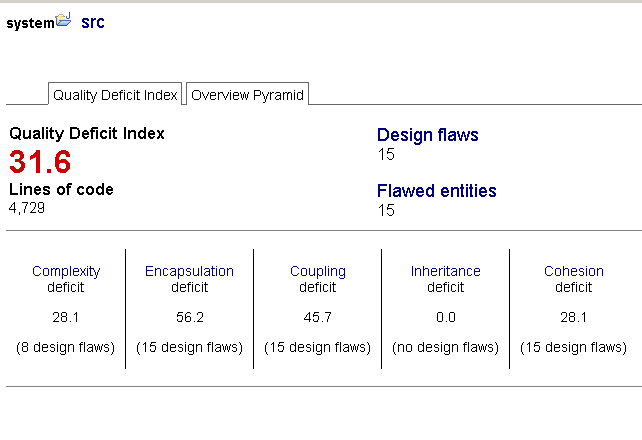
\includegraphics[scale=0.7]{infusion1.PNG}
\end{center}
\caption{Pre Re-factoring using Infusion}
\label{fig:infusion1}
\end{figure}

\begin{figure} [H]
\begin{center}
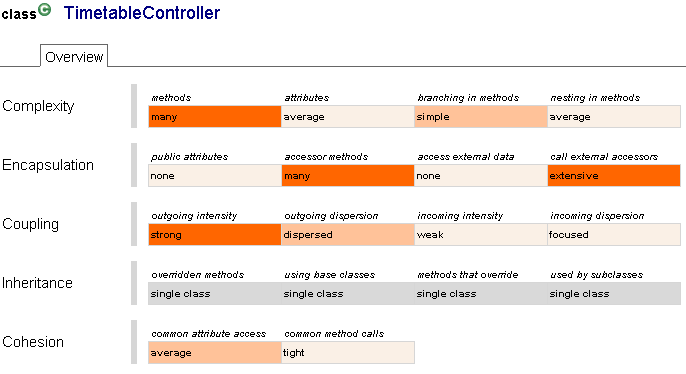
\includegraphics[scale=0.7]{infusion3.PNG}
\caption{Example of Class 'Bad Code Smell' Breakdown using Infusion}
\end{center}
\end{figure}

\begin{figure}[H]
\begin{center}
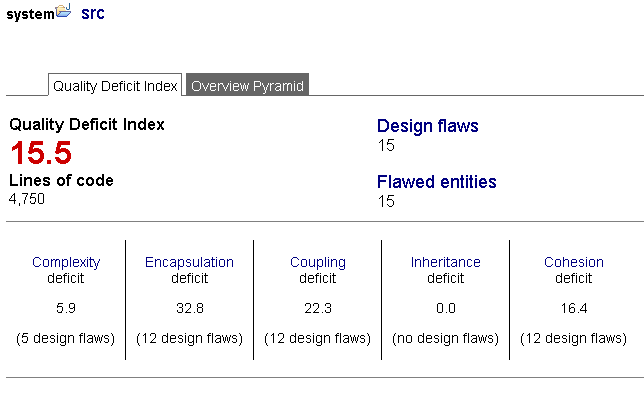
\includegraphics[scale=0.7]{infusion2.PNG}
\caption{Post Re-factoring using Infusion}
\end{center}
\end{figure}

While this tool was useful in terms of finding potential issues, it was difficult to know how good, or bad, my application was. There was no threshold identified by the application, and a score of 42.5, as shown in Figure~\ref{fig:infusion1}, does not carry much weight if I have no benchmark to compare it against. 

\subsection{Visualisations}

\subsubsection{CodeCity}

The software used to visualise the code was CodeCity, available at \hyperref[Code City]{http://www.inf.usi.ch/phd/wettel/codecity.html}. In order to run CodeCity, a MSE file needed to be created by inFusion. The CodeCity application reads this file, and represents your code as a city. The city is broken down into blocks, defined by a package, and within each block, there are a number of buildings, that represent classes. The size of the building is related to the size and complexity of the class it represents. Figures~\ref{fig:2dcc} and~\ref{fig:3dcc} show the 2D and 3D representations of the application created for this project. 
 
\begin{figure}[H]
\begin{center}
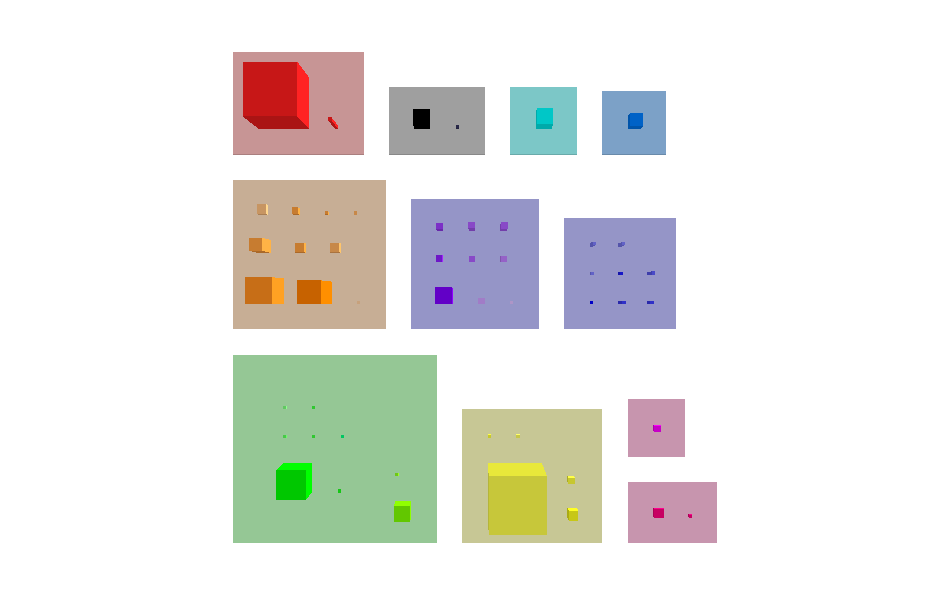
\includegraphics[scale=0.5]{codecity2d.png}
\caption{CodeCity 2D Visualisation of Application}
\label{fig:2dcc}
\end{center}
\end{figure}

\begin{figure}[H]
\begin{center}
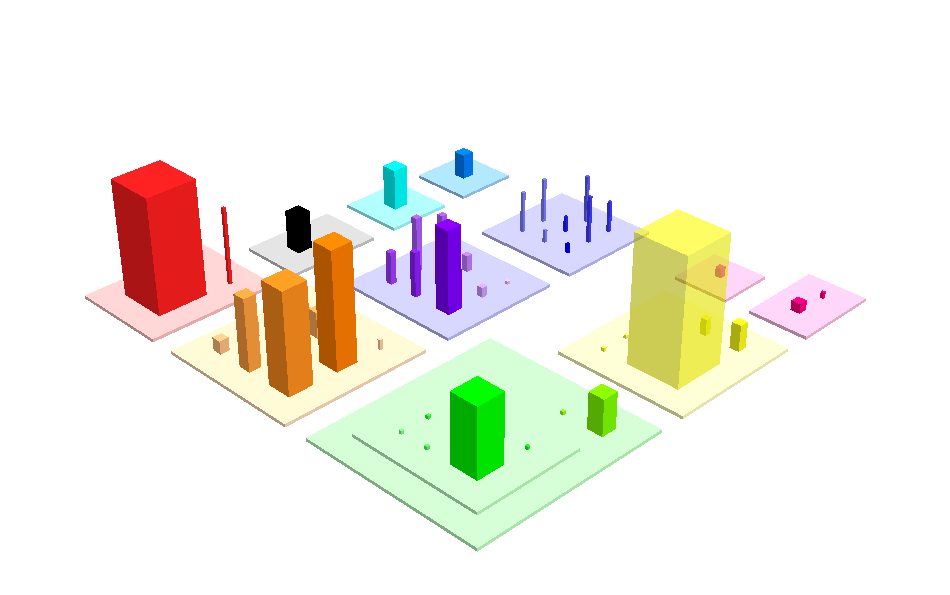
\includegraphics[scale=0.5]{codecity3d.png}
\caption{CodeCity 3D Visualisation of Application}
\label{fig:3dcc}
\end{center}
\end{figure}

Visualisation is a quick way to highlight potential issues and bad code smells, such as data classes, by looking at the size of a building. While this does not fix any problems, it aids in drawing attention to potential issues through the development cycle. 

\subsubsection{Gource}

Gource is an open source version control visualisation tool. It visualises the work flow of an application by using the commits with a git repository. This was useful in showing how the application came together, the timeline of the work areas within the project, such as the creation of controllers, dao and service layers, and how the nature of the project changed from one of creation to modification. The source for this application is available at \textit{https://code.google.com/p/gource/}.

The tool is run from a command line prompt with ffmpeg, a video encoding tool, used to convert the output from Gource to a wmv file. The commands used are illustrated in Figure~\ref{fig:gourcecmd}.
\newpage
\begin{lstlisting}
gource -1024x768 --stop-position 1.0 --highlight-all-users --hide-filenames --seconds-per-day 5 --output-framerate 60 --output-ppm-stream output.ppm
ffmpeg -y -r 60 -f image2pipe -vcodec ppm -i output.ppm  -vcodec wmv1 -r 60 -qscale 0 out.wmv
\end{lstlisting}
\begin{figure}
\caption{Commands for Gource output}
\label{fig:gourcecmd}
\end{figure}

The image in Figure~\ref{fig:gource} is a snapshot from the video output.

\begin{figure}[H]
\begin{center}
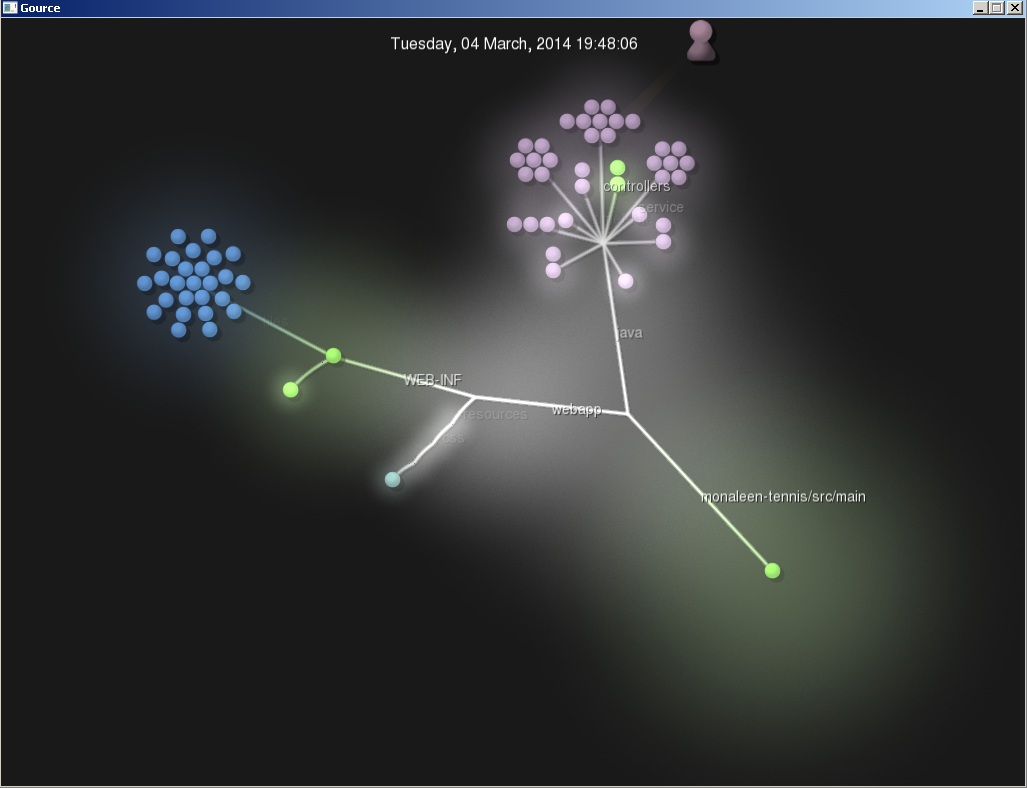
\includegraphics[scale=0.45]{gource.png}
\caption{Gource Snapshot}
\label{fig:gource}
\end{center}
\end{figure}

The output file is current hosted at http://youtu.be/Ct1E4jcmPKE.

